\chapter{Wavetable ohne Modifier}
\section{}
Die Länge des Wavetables zur Erzeugung eines White Tones mit Grundfrequenz $f0$ = 100 Hz bei einer Abtatsfrequenz von $f_s$ = 44100 Hz ergibt sich durch die Formel $N = \frac{f_s} {f_0}$. In unserem Fall ist $N$ = 441. 
\section{}
Der Wavetable wird mit Zufallszahlen zwischen -1 und 1 aufgefüllt. Zur Erzeugung der wav-Dateien wird der Karplus-Strong Algorithmus verwendet: Um ein drei Sekunden langes Signal bei einer Abtastfrequenz von $f_s$ = 44100 Hz zu erzeugen muss der Wavetable $n = \frac{N_{\mathrm{signal}}}{N} = \frac{3s \cdot 44100Hz}{441} = 300$ mal aneinander gereiht werden.
\section{}
In den mittels FFT erhaltenen Betragsspektren der Signale ist die charakteristische Obertonstruktur für White Tones deutlich zu erkennen. Es kommen lediglich Frequenzanteile bei der Grundfrequenz von 100 Hz und ihren ganzzahligen Vielfachen (Obertöne) vor. Die Amplituden der einzelnen Frequenzen sind zufällig bzw. werden durch die in den drei verschiedenen Wavetables individuell generierten Zufallssignale determiniert. Die Spektren setzen sich in gleicher Weise über den bis 2000 Hz dargestellten Frequenzbereich hinaus bis zur halben Abstastfrequenz von 22050 Hz fort. Zur einheitlichen Normalisierung der Spektren wurde die maximale Amplitude aller drei Betragsspektren als Normalisierungsfaktor verwendet.\newline 
\includegraphics[width = 0.7\textwidth]{spectrum1}
\newline
\includegraphics[width = 0.7\textwidth]{spectrum2}
\newline
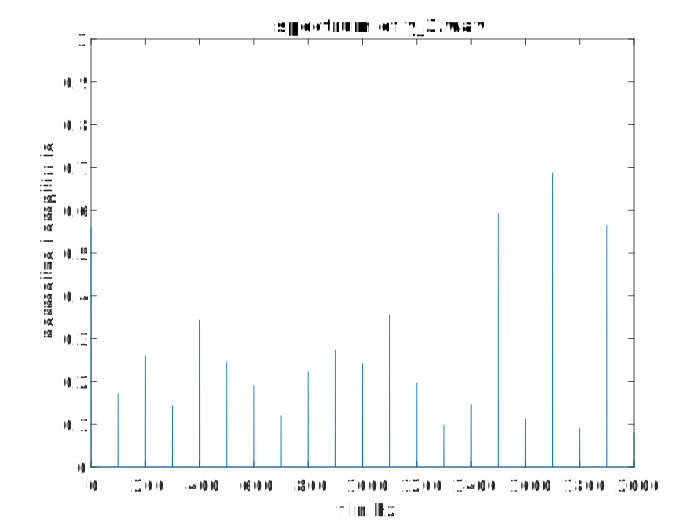
\includegraphics[width = 0.7\textwidth]{spectrum3}